\chapter{Quantum Bayesian Formalism and Quadratic Speedup via QAE}\label{chap:quantum_bayesian_formalism}

Having rigorously established the classical computational barriers of Bayesian inference in Chapter \ref{chap:classical_limits}---specifically the exponential treewidth memory ceiling $\mathcal{O}(N \cdot d^{w+1})$ and the asymptotic sampling divergence $\mathrm{RE} \to \infty$ for rare astrobiological events---this chapter establishes the mathematical framework of the proposed quantum solution. To circumvent these bottlenecks, we transition from classical probability theory (governed by discrete real-valued probability vectors, stochastic matrices, and the Kolmogorov axioms) to the geometric formalism of quantum mechanics (governed by continuous complex probability amplitudes within a finite-dimensional Hilbert space). This transition translates graphical causality into unitary quantum operators, replacing classical tabulation with quantum superposition and entanglement.

\section{Quantum Bayesian Networks (QBN): Hilbert Space and Amplitude Encoding}\label{sec:qbn_amplitude_encoding}

The physical implementation of a Quantum Bayesian Network (QBN) requires mapping the coupled photochemical dependencies of an exoplanetary atmosphere directly into the quantum state of a register of qubits \cite{low2014}. This section details the axiomatic foundations of this transition, the topological compilation of causal Directed Acyclic Graphs (DAGs) into quantum circuits, and the mathematical derivation of the Amplitude Encoding protocol.

\subsection{Axiomatic Formulation of Quantum Probability in Hilbert Spaces}
Classical Bayesian networks operate within a Kolmogorov probability space $(\Omega, \mathcal{F}, P)$, where random variables representing physical parameters (e.g., the atmospheric concentration of methane, $\mathrm{CH}_4$) are defined by discrete probability distributions constrained by the $L_1$ norm ($\sum_x P(x) = 1$). When multiple variables are conditionally coupled, representing their joint state demands explicitly tabulating every permutation in a multi-dimensional Cartesian product, inevitably precipitating the exponential treewidth explosion $\mathcal{O}(N \cdot d^{w+1})$.

\notatfm{\textbf{Hilbert Space:} Quantum probability vectors reside in an $L_2$-normalized Hilbert space $\mathcal{H} = \bigotimes_{i=1}^n \mathcal{H}_i$, storing $2^n$ joint states in $n$ qubits.}
Quantum mechanics reformulates this framework through the Dirac-von Neumann axioms \cite{nielsen2010}. A quantum system composed of $n$ qubits does not store a discrete list of disjoint probabilities. Instead, its state is described by a normalized state vector $\ket{\psi}$ residing within a $2^n$-dimensional complex Hilbert space:
\begin{equation}
\mathcal{H} = \mathcal{H}_1 \otimes \mathcal{H}_2 \otimes \dots \otimes \mathcal{H}_n = \mathbb{C}^{2^n}.
\label{eq:hilbert_space_tensor_product}
\end{equation}

The state vector is a linear superposition of computational basis states $\ket{x} \in \{0, 1\}^n$:
\begin{equation}
\ket{\psi} = \sum_{x=0}^{2^n-1} \alpha_x \ket{x}, \quad \alpha_x \in \mathbb{C}.
\label{eq:quantum_superposition_ch3}
\end{equation}
Unlike classical probability, probability amplitudes $\alpha_x$ are governed by the $L_2$ norm. The probability $P(x)$ of measuring a specific planetary configuration $\ket{x}$ is strictly dictated by Born's Rule:
\begin{equation}
P(x) = |\langle x \mid \psi \rangle|^2 = |\alpha_x|^2, \quad \text{subject to } \sum_{x=0}^{2^n-1} |\alpha_x|^2 = 1.
\label{eq:born_rule_ch3}
\end{equation}

When incorporating epistemic noise or missing observational telemetry from spaceborne observatories, our knowledge of an atmosphere is often an ensemble of pure states rather than an isolated vector. To accommodate this, we invoke the Density Matrix operator $\rho$:
\begin{equation}
\rho \equiv \sum_i p_i \ket{\psi_i}\bra{\psi_i}, \quad \mathrm{Tr}(\rho) = 1, \quad \rho \ge 0,
\label{eq:density_matrix_def_ch3}
\end{equation}
where $p_i \ge 0$ represents the classical probability that the exoplanetary system occupies the pure quantum state $\ket{\psi_i}$. This density matrix formalism provides the theoretical basis for modeling open-system environmental decoherence and thermal relaxation on physical quantum hardware, as experimentally evaluated in Chapter \ref{chap:system_architecture} and subsequent chapters.

\subsection{Topological Mapping: From Directed Acyclic Graphs to Quantum Circuits}
Before quantum algorithms can process astrobiological data, the classical Bayesian structure $\mathcal{B} = (\mathcal{G}, \Theta)$ must be translated into an executable quantum circuit. In a quantum processor, information propagates forward through unitary operators. Because quantum gates must be unitary ($U^\dagger U = I$) and the No-Cloning Theorem forbids the copying of arbitrary unknown quantum states \cite{nielsen2010}, the circuit cannot be assembled arbitrarily.

\notatfm{\textbf{Topological Sort:} The causal DAG must be topologically sorted ($\pi$) so that parent qubits are fully prepared before acting as controls for child nodes.}
The compilation pipeline requires computing a strict \emph{Topological Sort} $\pi$ of the DAG $\mathcal{G} = (V, E)$. This algorithmic ordering ensures that for every directed edge $(u, v) \in E$, the parent node $u$ strictly precedes the child node $v$ in the execution schedule:
\begin{equation}
(u, v) \in E \implies \pi(u) < \pi(v).
\label{eq:topological_sort_condition}
\end{equation}

This causal ordering is deeply anchored in the local Markov condition: a variable $X_i$ is conditionally independent of its non-descendants given its direct parent set $\mathrm{Parents}(X_i)$. In our quantum circuit architecture, this dictates that the unitary operator $U(X_i)$ applied to the target qubit representing variable $X_i$ is controlled exclusively by the qubits representing $\mathrm{Parents}(X_i)$:
\begin{equation}
U(X_i) = \sum_{k \in \mathrm{states}(\mathrm{Parents}(X_i))} \left(\ket{k}\bra{k}\right)_{\mathrm{Parents}(X_i)} \otimes R_y\left(\theta_{i \mid k}\right)_{X_i}.
\label{eq:topological_cpt_unitary}
\end{equation}

Importantly, to preserve circuit modularity and facilitate compilation into high-level gate libraries via Qiskit's \texttt{.to\_gate()} method, these subcircuits must never contain internal barrier directives (\texttt{qc.barrier()}). Barriers inhibit peephole optimization and break hierarchical transpilation across IBM Quantum backend target architectures.

\subsection{The Amplitude Encoding Protocol: Mathematical Derivation}
The mathematical core for mapping classical joint probability distributions into the Hilbert space is the Amplitude Encoding protocol, formulated for Bayesian networks by Low, Yoder, and Chuang (2014) \cite{low2014}. The computational objective is to synthesize a global unitary state preparation operator $\mathcal{A}$ that acts upon the $N$-qubit vacuum state $\ket{0}^{\otimes N}$, producing a coherent superposition whose amplitudes are the square roots of the classical Joint Probability Distribution:
\begin{equation}
\ket{\Psi} = \mathcal{A}\ket{0}^{\otimes N} = \sum_{x \in \{0,1\}^N} \sqrt{P(X_1=x_1, \dots, X_N=x_N)} \ket{x_1 x_2 \dots x_N}.
\label{eq:amplitude_encoding_state_ch3}
\end{equation}

The operator $\mathcal{A}$ decomposes into a sequential product of local unitary operators ordered by the topological sort: $\mathcal{A} = U_N U_{N-1} \dots U_1$. The elementary building block of each transformation is the parameterized Pauli-Y rotation gate:
\begin{equation}
R_y(\theta) \equiv \exp\left(-i \frac{\theta}{2} Y\right) = \begin{pmatrix} \cos(\theta/2) & -\sin(\theta/2) \\ \sin(\theta/2) & \cos(\theta/2) \end{pmatrix}.
\label{eq:ry_matrix_ch3}
\end{equation}

\subsubsection{Root Node Initialization}
For a root variable $X_r$ with no incoming causal edges ($\mathrm{Parents}(X_r) = \emptyset$, such as stellar spectral type or orbital habitable zone location), the prior probability $P(X_r = 1)$ is encoded into its qubit via an unconditional $R_y(\theta_r)$ rotation. Setting the rotation angle to:
\begin{equation}
\theta_r = 2 \arcsin\left(\sqrt{P(X_r = 1)}\right),
\label{eq:root_rotation_angle}
\end{equation}
the action of the gate on the ground state $\ket{0}$ yields:
\begin{equation}
R_y(\theta_r)\ket{0} = \cos\left(\frac{\theta_r}{2}\right)\ket{0} + \sin\left(\frac{\theta_r}{2}\right)\ket{1} = \sqrt{P(X_r=0)}\ket{0} + \sqrt{P(X_r=1)}\ket{1}.
\label{eq:root_node_rotation_ch3}
\end{equation}

\subsubsection{Child Node Conditional Rotations}
For dependent variables (child nodes) influenced by parent variables $\mathrm{Parents}(X_j)$, conditional probabilities are encoded using multi-controlled rotation gates $C^k(R_y)$. The unitary operator for variable $X_j$ is given by:
\begin{equation}
U(X_j) = \sum_{k \in \{0,1\}^{|\mathrm{Parents}(X_j)|}} \left(\ket{k}\bra{k}\right)_{\mathrm{Parents}(X_j)} \otimes R_y\left(2 \arcsin\left(\sqrt{P(X_j=1 \mid \mathrm{Parents}(X_j)=k)}\right)\right)_{X_j}.
\label{eq:child_node_multicontrolled_ry}
\end{equation}
The projector $\ket{k}\bra{k}$ selectively activates the rotation on qubit $X_j$ if and only if the parent register occupies classical configuration $k$. In modern Qiskit implementations, these operations are synthesized via the object-oriented pattern \texttt{RYGate(theta).control(num\_ctrl\_qubits)}, completely deprecating legacy functions like \texttt{qc.mcry()}.

To transpile these multi-controlled gates onto physical hardware supporting only 1-qubit and 2-qubit native gates, we deploy the decomposition theorem of Barenco et al.~(1995) \cite{barenco1995}. A $k$-controlled unitary operation $C^k(U)$ is compiled into an equivalent network of single-qubit rotations and $\mathcal{O}(2^k)$ CNOT gates (or $\mathcal{O}(k)$ using borrowable dirty ancilla qubits).

\subsection{Resolution of the Spatial Bottleneck: Rigorous Proof of Advantage}
The primary structural advantage of this Amplitude Encoding protocol is its exponential spatial compression over classical exact inference.

In classical Bayesian networks, exact inference via Variable Elimination or the Junction Tree Algorithm requires storing and multiplying intermediate multi-dimensional clique tensors, leading to the spatial memory bound derived in Equation \eqref{eq:jta_treewidth_bound_ch2}:
\begin{equation}
\mathcal{M}_{\mathrm{classical}} = \mathcal{O}\left(N \cdot d^{w+1}\right).
\end{equation}
When dense atmospheric feedback loops cause the treewidth $w$ to approach $N-1$, classical RAM saturation occurs exponentially.

\notatfm{\textbf{Spatial Compression Bound:} An $N$-qubit register stores $2^N$ joint probabilities in $\mathcal{O}(N)$ space. State preparation requires only $\mathcal{O}(N \cdot 2^{k_{\max}})$ gates.}
Conversely, by mapping the entire $2^N$-dimensional joint probability distribution into the continuous probability amplitudes of an $N$-qubit quantum register, the physical memory requirement scales strictly linearly:
\begin{equation}
\mathcal{M}_{\mathrm{quantum}} = \mathcal{O}(N) \text{ physical qubits}.
\label{eq:quantum_spatial_bound}
\end{equation}

Furthermore, the temporal complexity required to prepare this state avoids arbitrary state preparation blowup ($\mathcal{O}(2^N)$). As established by Low et al.~(2014) \cite{low2014}, the number of elementary gates required to synthesize $\mathcal{A}$ depends strictly on the maximum parent in-degree of the DAG:
\begin{equation}
k_{\max} \equiv \max_{i \in \{1, \dots, N\}} |\mathrm{Parents}(X_i)|.
\label{eq:max_in_degree_def}
\end{equation}
The gate synthesis complexity is bounded by:
\begin{equation}
\mathcal{C}_{\mathrm{prep}} = \sum_{i=1}^N 2^{|\mathrm{Parents}(X_i)|} = \mathcal{O}\left(N \cdot 2^{k_{\max}}\right).
\label{eq:state_prep_complexity_proof}
\end{equation}
For realistic astrobiological networks where each chemical species is directly influenced by at most $k_{\max} \le 3$ atmospheric parents, $2^{k_{\max}} \le 8$, and the state preparation complexity scales strictly linearly with the number of variables: $\mathcal{C}_{\mathrm{prep}} = \mathcal{O}(N)$.

\begin{figure}[htbp]
    \centering
    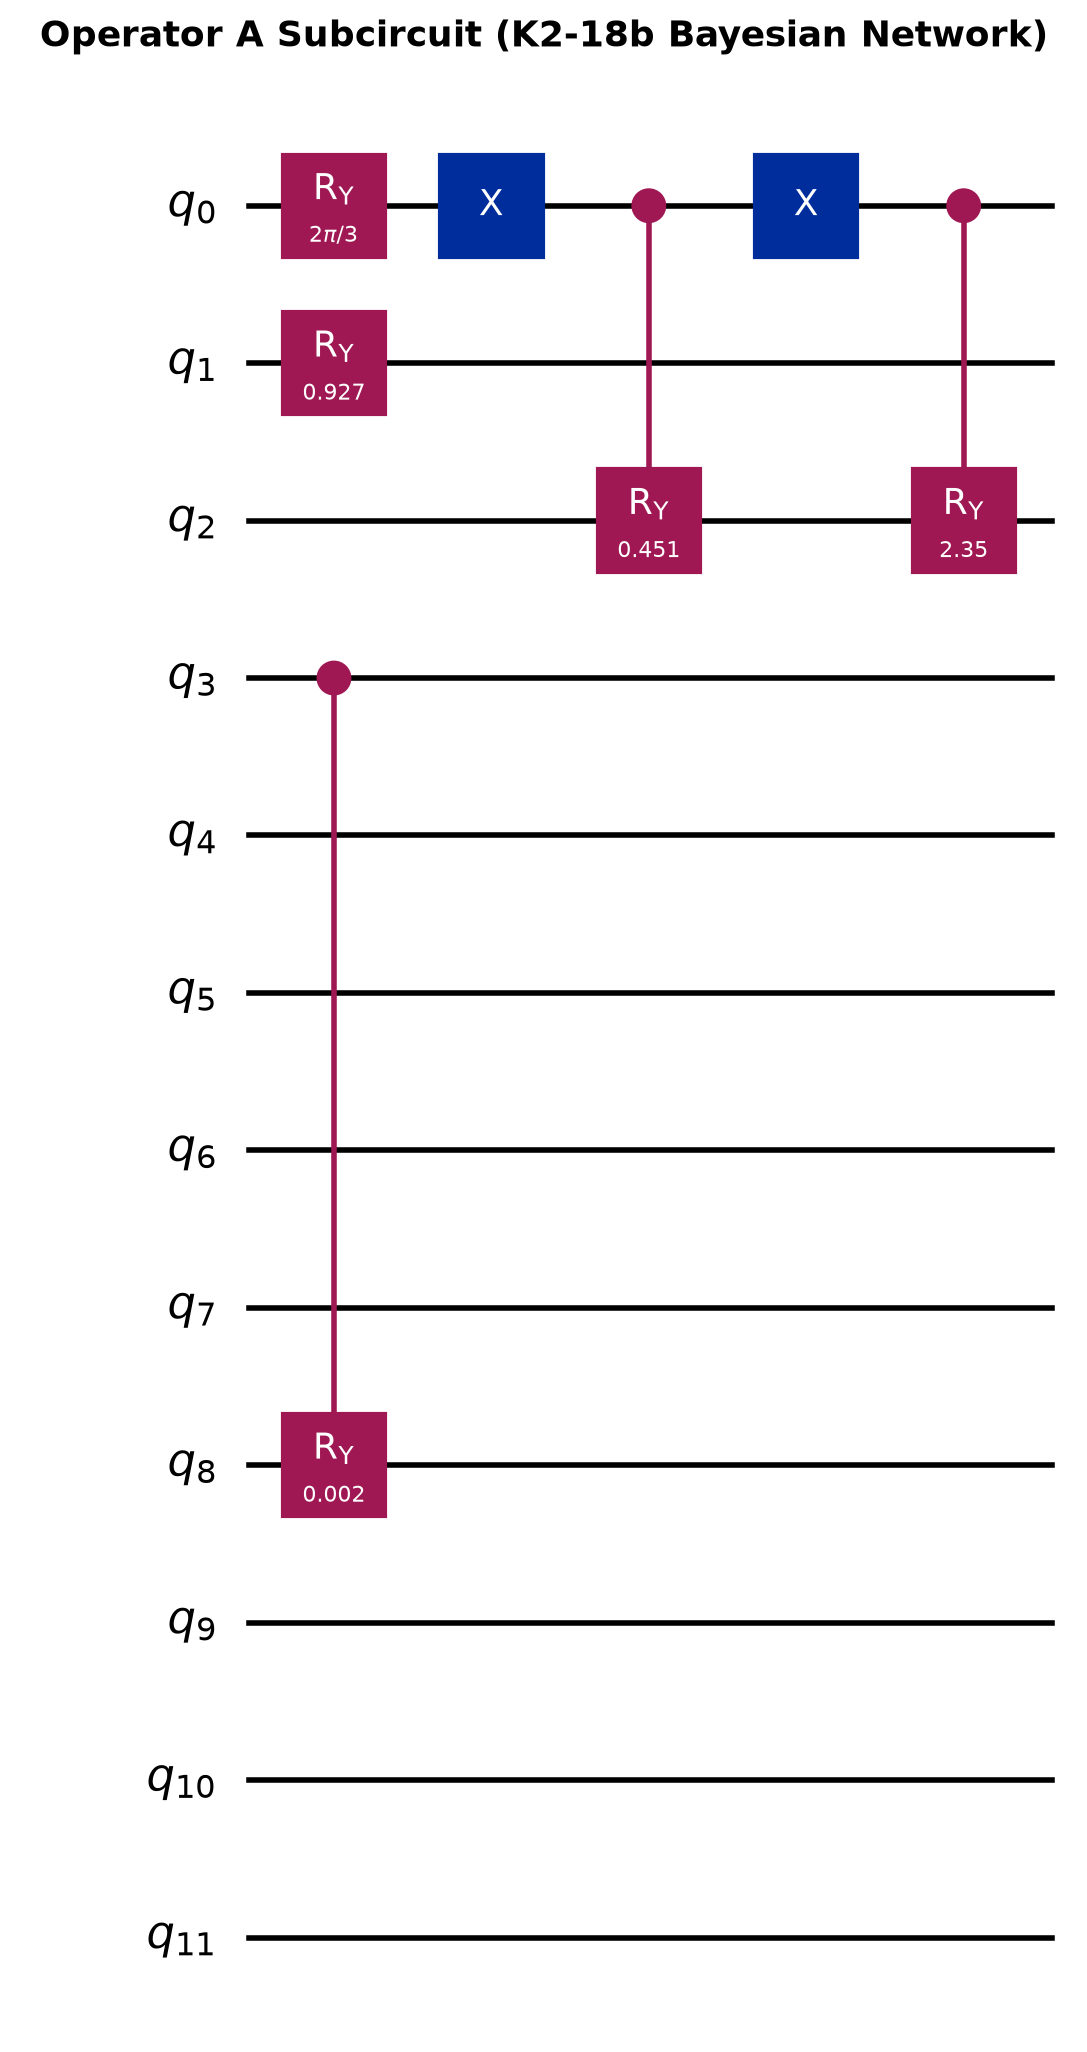
\includegraphics[width=0.70\textwidth, height=0.52\textheight, keepaspectratio]{figures/3.quantum_bayesian_formalism/circuit_operator_A.png}
    \caption{\textbf{Quantum Circuit Architecture of the State Preparation Operator $\mathcal{A}$.} Topological compilation of the causal Bayesian network into an $N$-qubit register. Root nodes are initialized via single-qubit $R_y(\theta)$ rotations, while hierarchical dependencies are encoded through a topological cascade of multi-controlled Pauli-Y rotations ($C^k(R_y)$), establishing conditional entanglement without internal barriers.}
    \label{fig:circuit_operator_A}
\end{figure}

As depicted in Figure \ref{fig:circuit_operator_A}, the state preparation operator $\mathcal{A}$ compiles the complete multi-gas dependency structure into a coherent, barrier-free quantum subcircuit.

\section{Quantum Amplitude Estimation (QAE): Geometric Deduction of Grover's Operator and Asymptotic Speedup}\label{sec:qae_derivation_speedup}

While Amplitude Encoding resolves the classical spatial memory bottleneck, extracting quantitative probabilities requires an active amplification protocol. As demonstrated in Chapter \ref{chap:classical_limits}, classical stochastic sampling (MCMC) suffers from an asymptotic convergence rate constrained to $\mathcal{O}(1/\sqrt{M})$ and exhibits catastrophic variance divergence ($\mathrm{RE} \to \infty$) for rare astrobiological events. This section presents a full geometric deduction of Quantum Amplitude Estimation (QAE), formulated by Brassard, H{\o}yer, Mosca, and Tapp (2002) \cite{brassard2002}, proving how QAE achieves the Heisenberg-limited convergence rate $\mathcal{O}(1/M)$.

\subsection{The Measurement Bottleneck in Unamplified Superpositions}
Direct projective measurement of the unamplified state $\ket{\Psi} = \mathcal{A}\ket{0}^{\otimes N}$ in the computational basis collapses the state according to Born's Rule. For an ultra-rare event---such as an industrial chlorofluorocarbon (CFC) technosignature with true posterior probability $a = 10^{-6}$---the probability of collapsing into the target state is:
\begin{equation}
P(\mathrm{target}) = |\langle x_{\mathrm{target}} \mid \Psi \rangle|^2 = a \approx 10^{-6}.
\end{equation}
Directly measuring $\ket{\Psi}$ reduces the quantum processor to classical random sampling. To achieve statistical confidence, the researcher must repeat circuit executions and measurements millions of times, recovering the classical standard error scaling $\sigma = \mathcal{O}(1/\sqrt{M})$. To achieve a quantum advantage, the algorithm must deterministically amplify the target state's amplitude before measurement.

\subsection{Geometric Parameterization of the Bipartite Hilbert Space}
Let $\chi: \{0, 1\}^N \to \{0, 1\}$ denote a Boolean oracle function that identifies the target astrobiological hypothesis (e.g., $\chi(x) = 1$ if configuration $x$ contains the desired biosignature or technosignature, and $\chi(x) = 0$ otherwise). This oracle partitions the $2^N$-dimensional Hilbert space $\mathcal{H}$ into two mutually orthogonal subspaces: the ``good'' target subspace $\mathcal{H}_1$ and the ``bad'' background subspace $\mathcal{H}_0$.

\notatfm{\textbf{2D Invariant Subspace:} The $2^N$-dimensional quantum state collapses geometrically into a 2D plane spanned by $\ket{\Psi_0}$ and $\ket{\Psi_1}$, parameterized by angle $\theta$.}
We define the normalized basis vectors for these subspaces as:
\begin{equation}
\ket{\Psi_1} \equiv \frac{1}{\sqrt{a}} \sum_{x: \chi(x)=1} \sqrt{P(x)} \ket{x}, \quad \ket{\Psi_0} \equiv \frac{1}{\sqrt{1-a}} \sum_{x: \chi(x)=0} \sqrt{P(x)} \ket{x},
\label{eq:bipartite_basis_ch3}
\end{equation}
where $a = \sum_{x: \chi(x)=1} P(x) \in [0, 1]$ is the exact cumulative probability of the target hypothesis. Because $\langle \Psi_0 \mid \Psi_1 \rangle = 0$, these two vectors span a two-dimensional invariant subspace that contains the initial state $\ket{\Psi}$. We can express $\ket{\Psi}$ purely as a geometric vector in this 2D plane parameterized by an angle $\theta$:
\begin{equation}
\ket{\Psi} = \cos(\theta) \ket{\Psi_0} + \sin(\theta) \ket{\Psi_1},
\label{eq:bipartite_state_angle_ch3}
\end{equation}
where the target probability is related to the geometric angle by:
\begin{equation}
a = \sin^2(\theta), \quad \theta = \arcsin(\sqrt{a}) \in \left[0, \frac{\pi}{2}\right].
\label{eq:theta_angle_relation}
\end{equation}
The computational challenge of probability estimation is thus transformed into the geometric problem of estimating the continuous phase angle $\theta$.

\\begin{figure}[htbp]
    \centering
    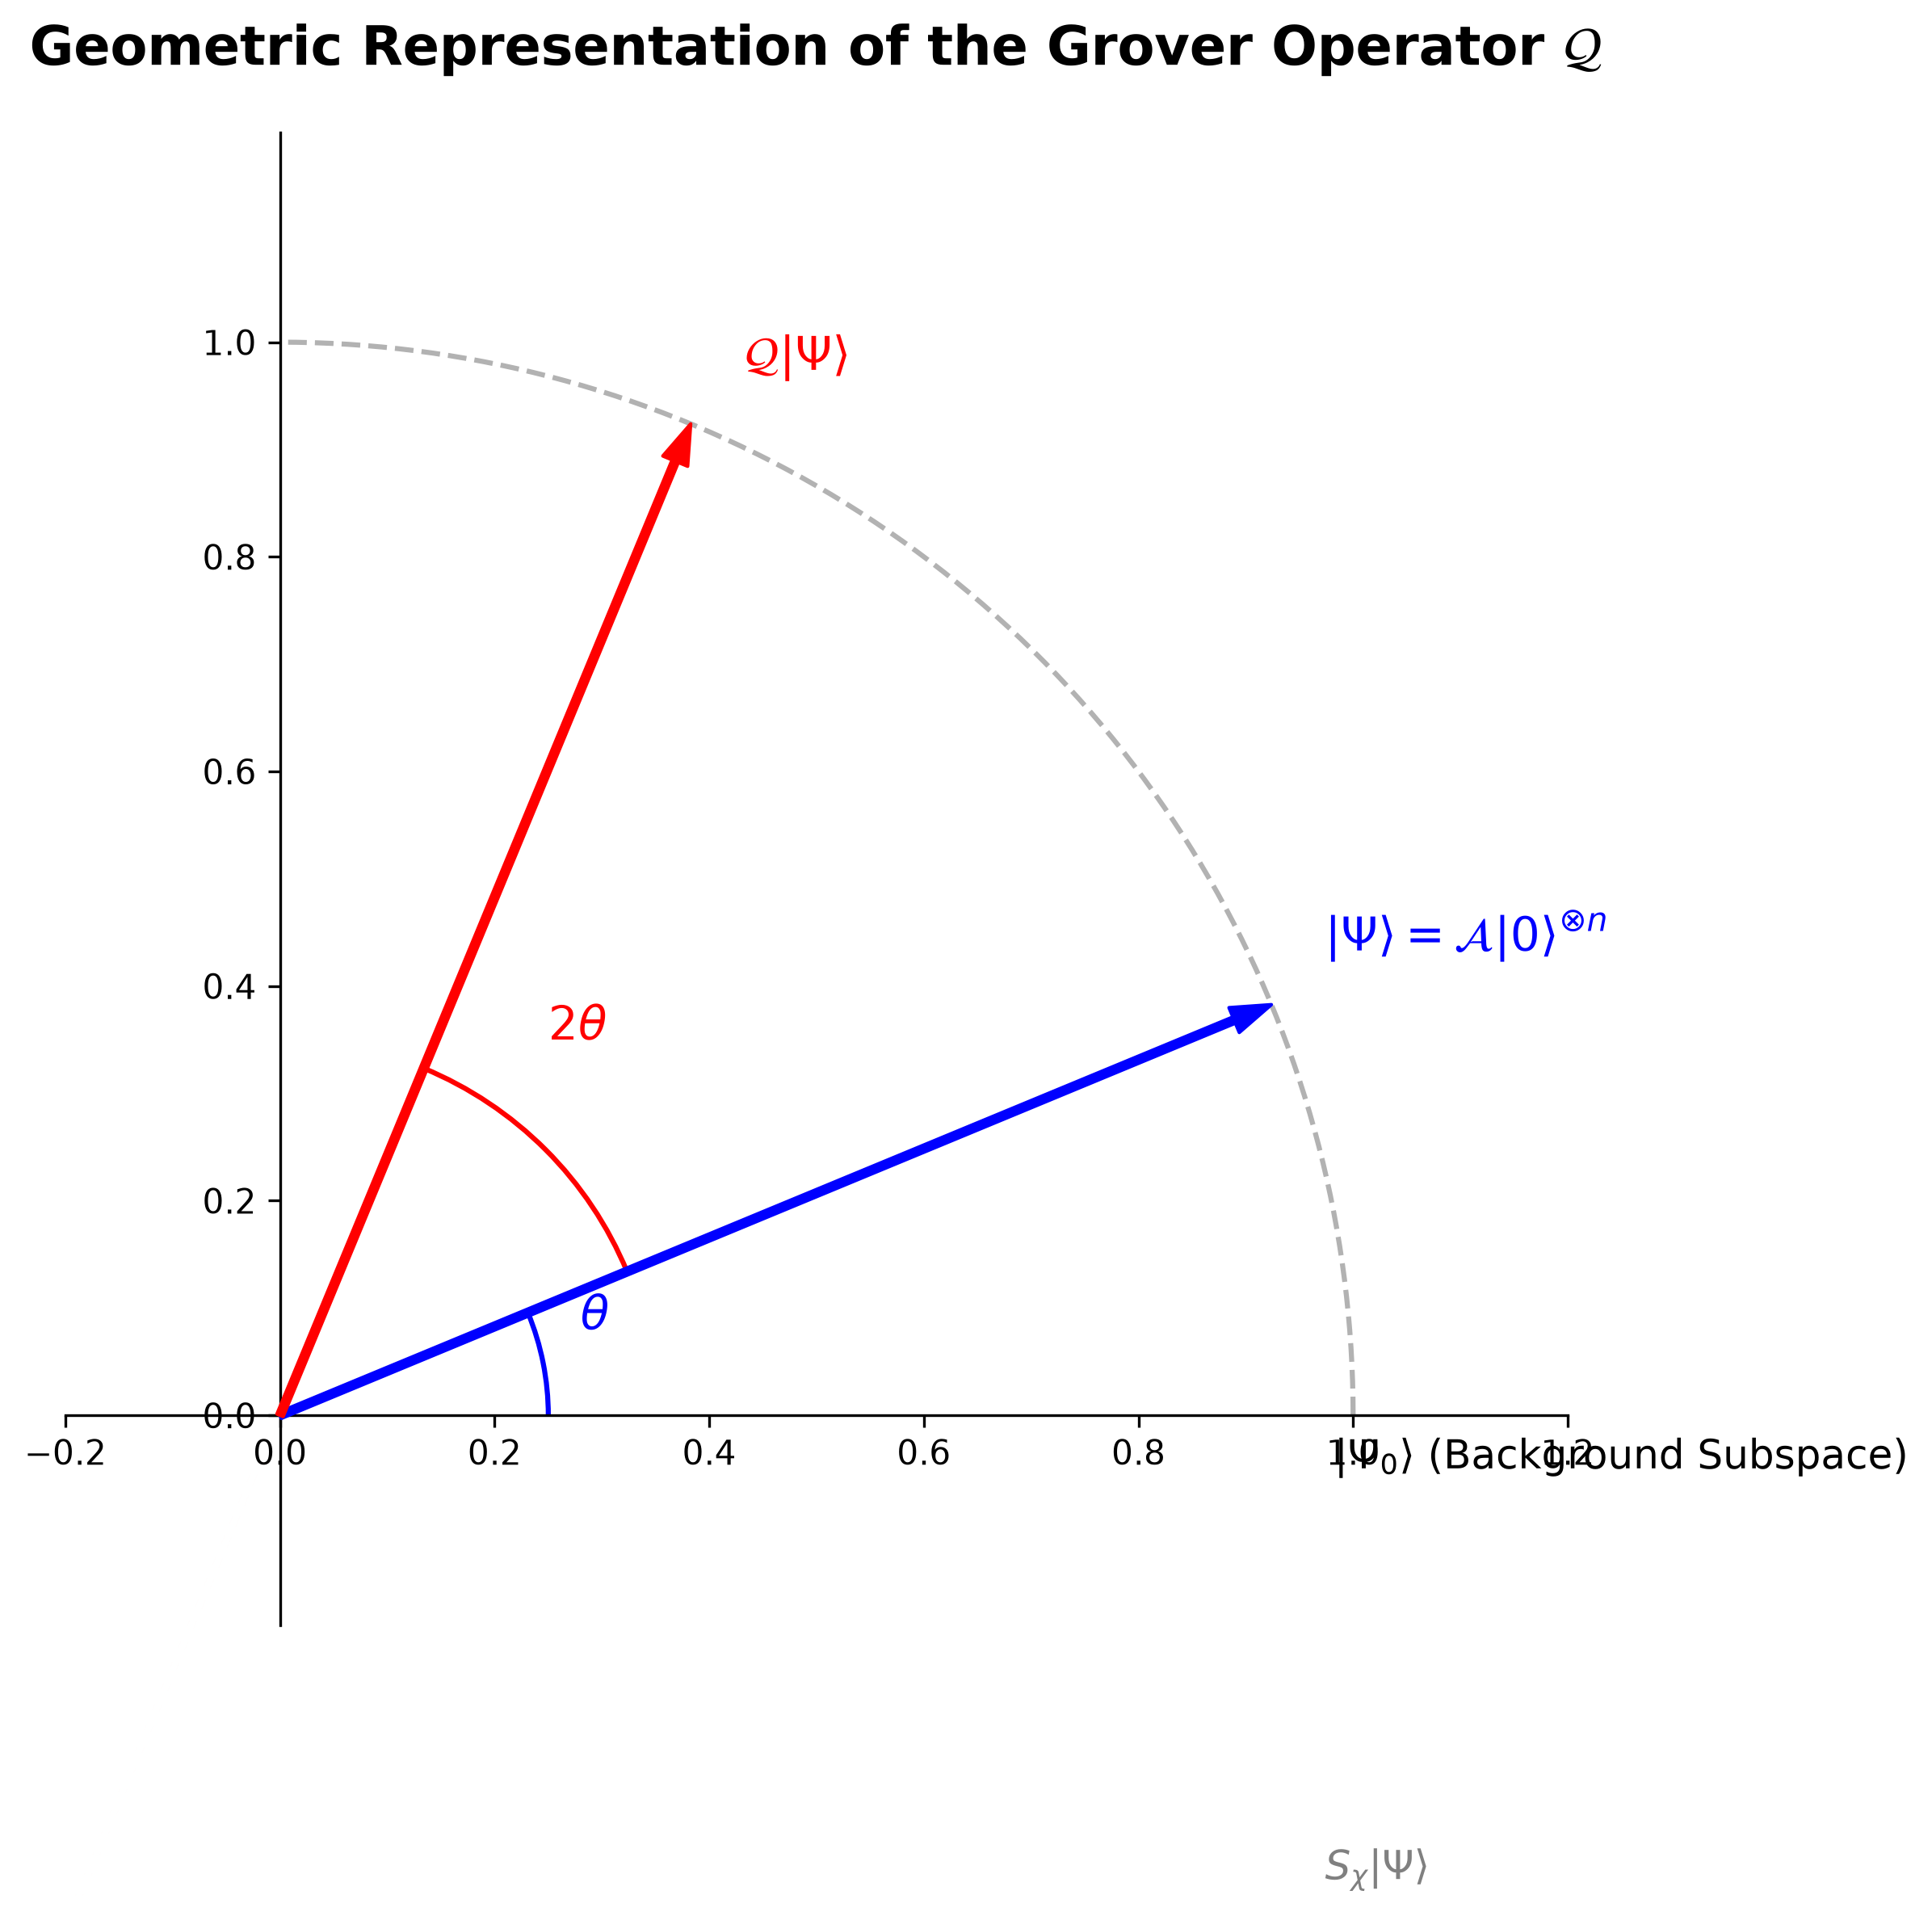
\includegraphics[width=0.65\textwidth, height=0.40\textheight, keepaspectratio]{figures/3.quantum_bayesian_formalism/figure_grover_geometry.png}
    \caption{\textbf{Geometric Representation of the Grover Operator $\mathcal{Q}$.} In the two-dimensional invariant subspace spanned by $|\Psi_0\rangle$ and $|\Psi_1\rangle$, the initial state vector $|\Psi\rangle$ resides at an angle $\theta$. The composite reflection $-\mathcal{A}S_0\mathcal{A}^\dagger S_\chi$ performs a deterministic counter-clockwise rotation by $2\theta$, amplifying the amplitude of the target subspace $|\Psi_1\rangle$.}
    \label{fig:grover_geometry}
\end{figure}

\subsection{Matrix Algebra of Grover's Iteration Operator \texorpdfstring{$\mathcal{Q}$}{Q}}
To amplify the amplitude of $\ket{\Psi_1}$ and measure $\theta$, the architecture deploys Grover's iteration operator $\mathcal{Q}$. The operator $\mathcal{Q}$ is defined as the composite product of two unitary reflections within the 2D subspace:
\begin{equation}
\mathcal{Q} \equiv -\mathcal{A} S_0 \mathcal{A}^\dagger S_\chi.
\label{eq:grover_operator_def_ch3}
\end{equation}

\begin{figure}[htbp]
    \centering
    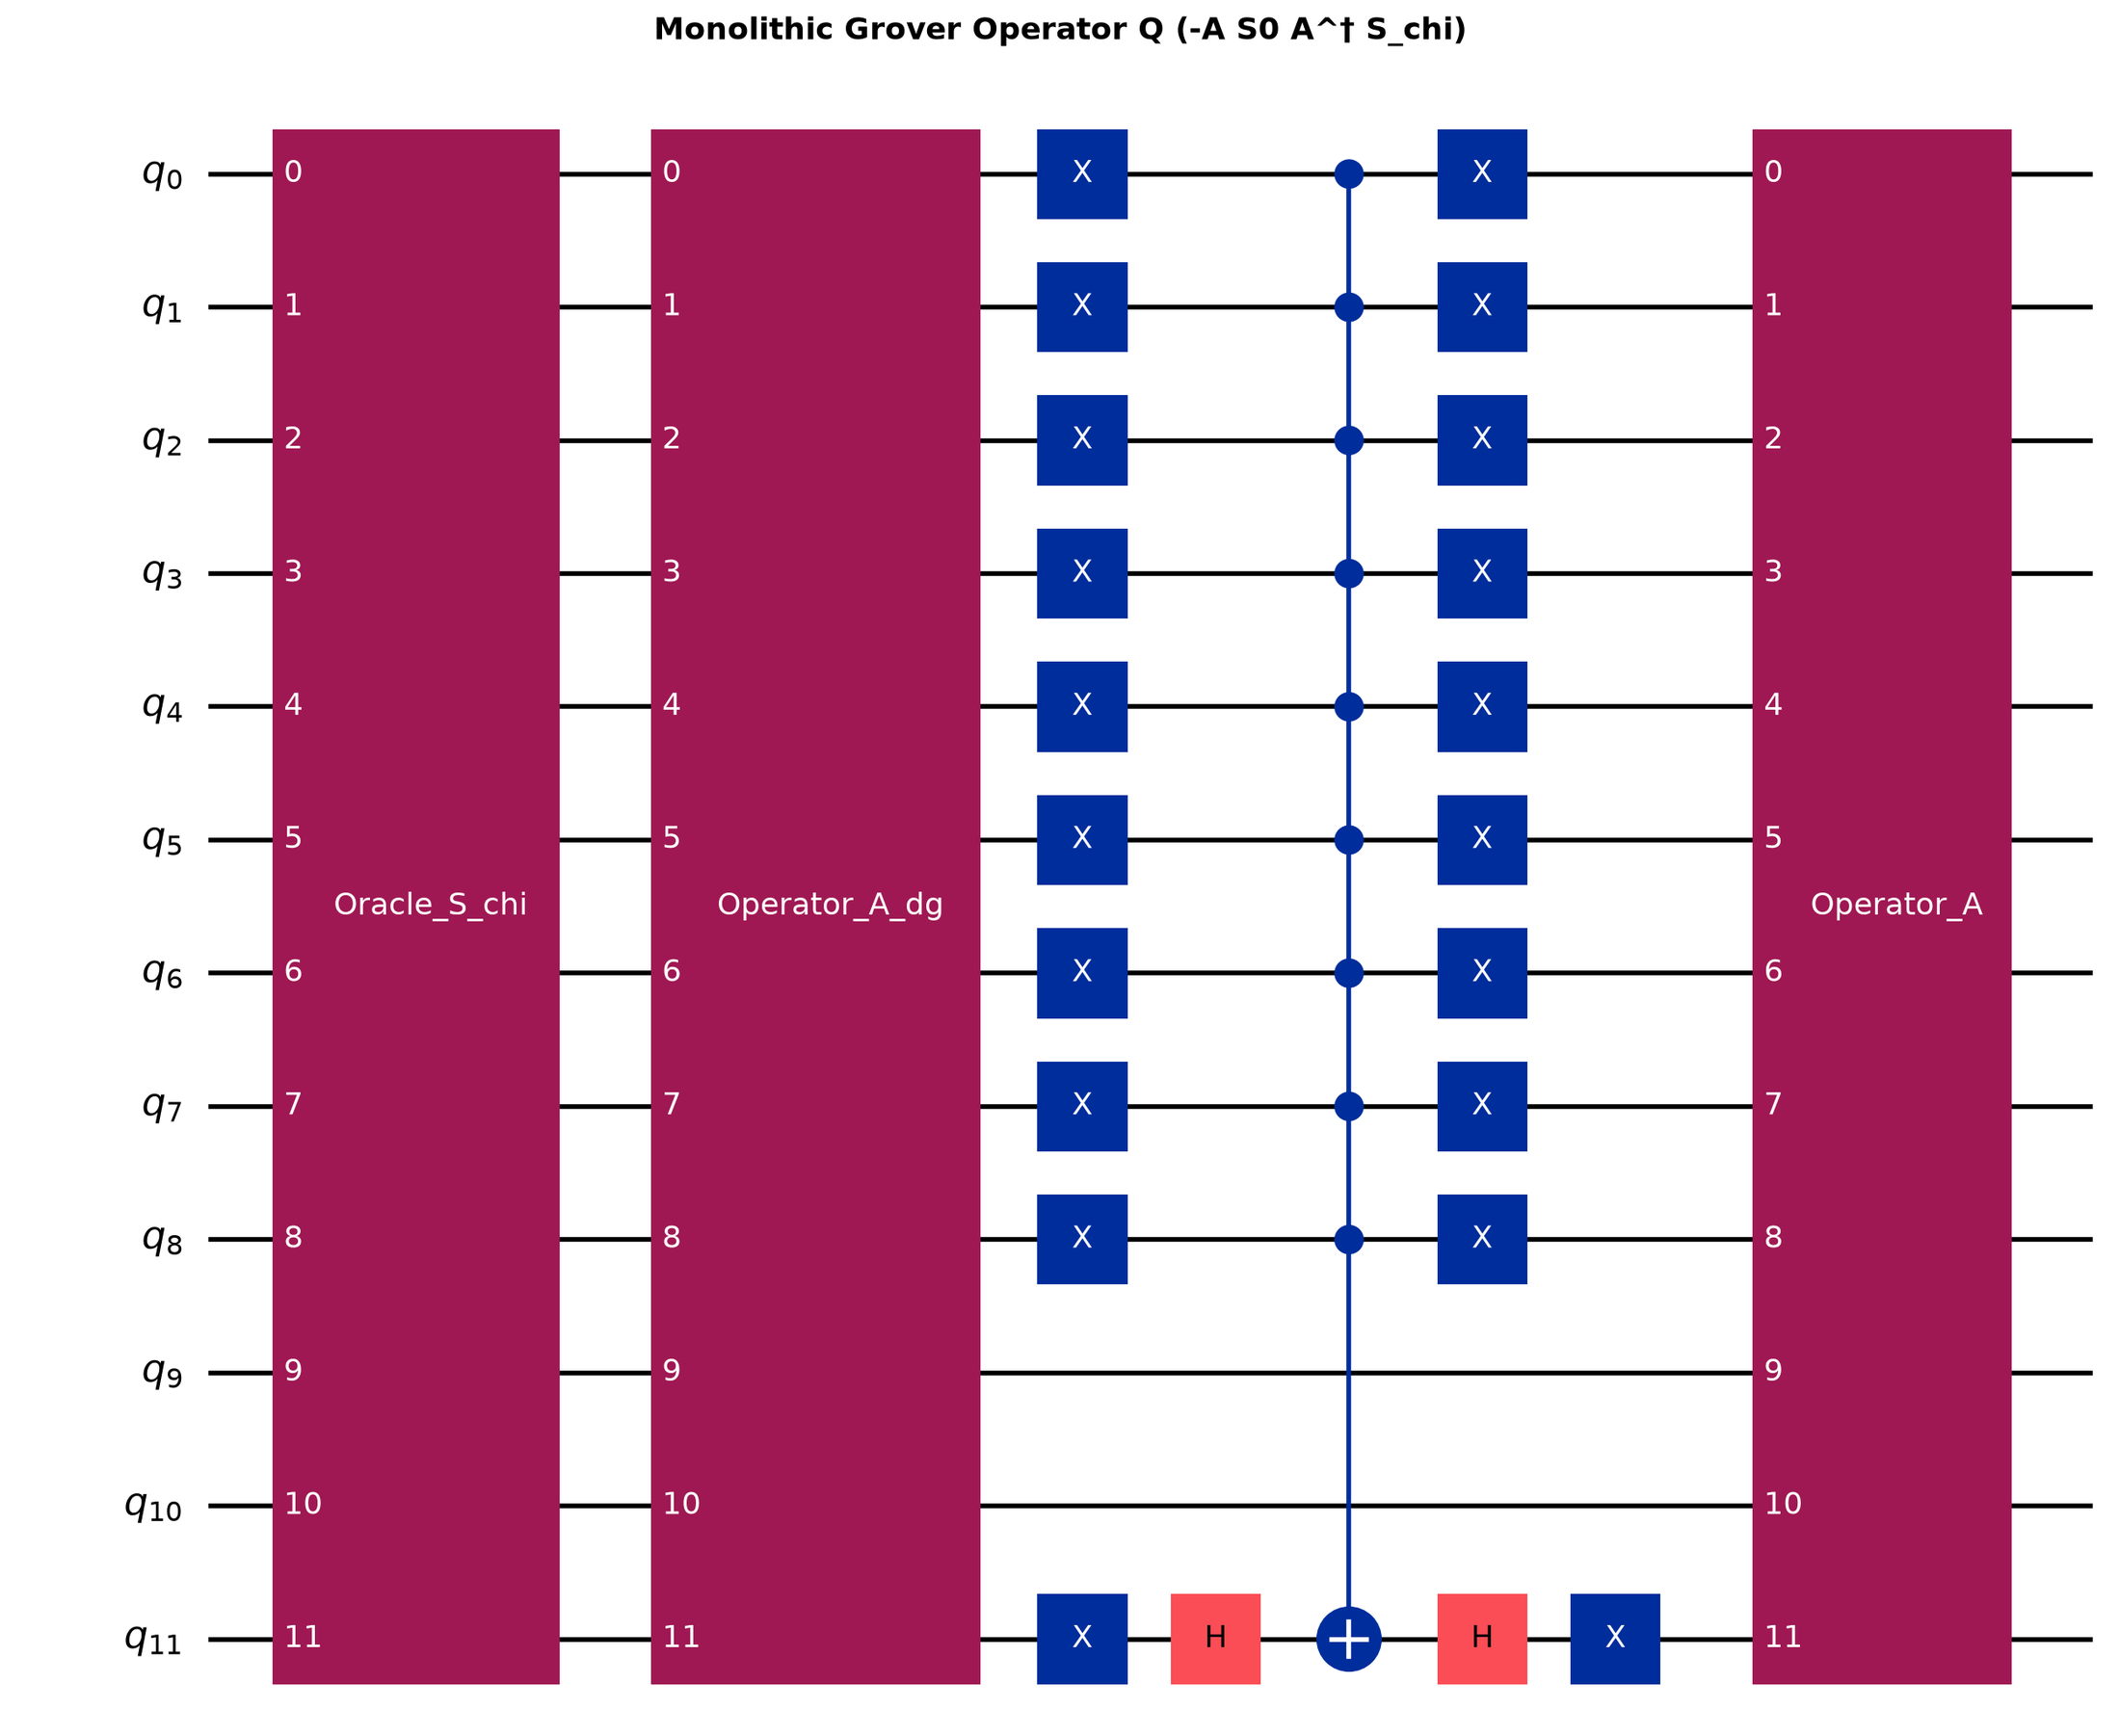
\includegraphics[width=0.85\textwidth, height=0.45\textheight, keepaspectratio]{figures/3.quantum_bayesian_formalism/circuit_operator_grover.png}
    \caption{\textbf{Quantum Circuit Architecture of the Grover Iteration Operator $\mathcal{Q}$.} The operator executes a phase inversion of marked target states ($S_\chi$), followed by inverse state preparation ($\mathcal{A}^\dagger$), zero-state phase reflection ($S_0$), and forward state preparation ($\mathcal{A}$), producing a deterministic $2\theta$ rotation in the bipartite plane.}
    \label{fig:circuit_operator_grover}
\end{figure}

The algebraic components of $\mathcal{Q}$ operate as follows:
\begin{enumerate}
    \item \textbf{Target Phase Oracle ($S_\chi$):} Inverts the phase of all basis states within the target subspace $\mathcal{H}_1$:
    \begin{equation}
    S_\chi = I - 2 \ket{\Psi_1}\bra{\Psi_1}.
    \label{eq:oracle_reflection_s_chi}
    \end{equation}
    Geometrically, $S_\chi$ reflects the state vector $\ket{\Psi}$ across the horizontal axis $\ket{\Psi_0}$.
    \item \textbf{Diffuse Reflection Operator ($-\mathcal{A} S_0 \mathcal{A}^\dagger$):} The zero-state phase reflection $S_0 = I - 2\ket{0}\bra{0}$, when conjugated by the state preparation operator $\mathcal{A}$, produces an inversion about the full state vector $\ket{\Psi}$:
    \begin{equation}
    -\mathcal{A} S_0 \mathcal{A}^\dagger = -\mathcal{A}\left(I - 2\ket{0}\bra{0}\right)\mathcal{A}^\dagger = 2\ket{\Psi}\bra{\Psi} - I.
    \label{eq:diffuse_reflection_operator}
    \end{equation}
\end{enumerate}

According to the Cartan-Dieudonn\'e theorem, the composition of two reflections across lines intersecting at an angle $\theta$ in a 2D Euclidean plane is a pure rotation by an angle of $2\theta$. Because the angle between the horizontal reflection axis $\ket{\Psi_0}$ and the state vector $\ket{\Psi}$ is $\theta$, a single application of $\mathcal{Q}$ rotates the state vector counter-clockwise by exactly $2\theta$:
\begin{equation}
\mathcal{Q}\ket{\Psi} = \cos(3\theta)\ket{\Psi_0} + \sin(3\theta)\ket{\Psi_1}.
\label{eq:single_grover_rotation_ch3}
\end{equation}
Applying $\mathcal{Q}$ recursively $j$ times deterministically yields:
\begin{equation}
\mathcal{Q}^j \ket{\Psi} = \cos((2j+1)\theta)\ket{\Psi_0} + \sin((2j+1)\theta)\ket{\Psi_1}.
\label{eq:j_grover_rotations_ch3}
\end{equation}
Figure \ref{fig:circuit_operator_grover} illustrates the full quantum circuit synthesis of this composite operator.

\subsection{Spectral Analysis and Eigenvalues of the \texorpdfstring{$\mathcal{Q}$}{Q}} Operator
To extract the continuous probability $a = \sin^2(\theta)$ without relying on destructive projective sampling, QAE performs spectral analysis on the Grover operator $\mathcal{Q}$. In the orthonormal basis $\{\ket{\Psi_0}, \ket{\Psi_1}\}$, the matrix representation of $\mathcal{Q}$ is:
\begin{equation}
\mathcal{Q} = \begin{pmatrix} \cos(2\theta) & -\sin(2\theta) \\ \sin(2\theta) & \cos(2\theta) \end{pmatrix}.
\label{eq:grover_matrix_2d_ch3}
\end{equation}

The characteristic equation $\det(\mathcal{Q} - \lambda I) = 0$ evaluates to:
\begin{equation}
\lambda^2 - 2\cos(2\theta)\lambda + 1 = 0.
\label{eq:grover_characteristic_equation}
\end{equation}
The roots of this quadratic equation are complex conjugate eigenvalues:
\begin{equation}
\lambda_\pm = \cos(2\theta) \pm i \sin(2\theta) = \exp(\pm i 2\theta).
\label{eq:grover_eigenvalues_ch3}
\end{equation}

The corresponding orthonormal eigenvectors are:
\begin{equation}
\ket{w_\pm} = \frac{1}{\sqrt{2}} \left( \ket{\Psi_0} \pm i \ket{\Psi_1} \right).
\label{eq:grover_eigenvectors_ch3}
\end{equation}
Expressing the initial state $\ket{\Psi}$ in this eigenbasis yields:
\begin{equation}
\ket{\Psi} = \frac{-i}{\sqrt{2}} \left( e^{i\theta}\ket{w_+} - e^{-i\theta}\ket{w_-} \right).
\label{eq:state_expansion_eigenbasis_ch3}
\end{equation}
Equation \eqref{eq:state_expansion_eigenbasis_ch3} establishes that applying $\mathcal{Q}$ to the quantum system imparts distinct phase shifts of $\pm 2\theta$ to the eigencomponents. Measuring this phase shift directly reveals $\theta$, and consequently the posterior probability $a = \sin^2(\theta)$.

\subsection{Quantum Phase Estimation (QPE) and the Inverse Quantum Fourier Transform (IQFT)}
To measure the eigenphase $\pm 2\theta$ coherently, QAE integrates the Grover operator within a Quantum Phase Estimation (QPE) circuit \cite{nielsen2010}. This requires an auxiliary evaluation register consisting of $m$ precision qubits initialized in an equal superposition via a cascade of Hadamard gates:
\begin{equation}
\ket{\phi_{\mathrm{eval}, 0}} = H^{\otimes m}\ket{0}^{\otimes m} = \frac{1}{\sqrt{M}} \sum_{y=0}^{M-1} \ket{y}, \quad M = 2^m.
\label{eq:evaluation_register_init}
\end{equation}

\begin{figure}[htbp]
    \centering
    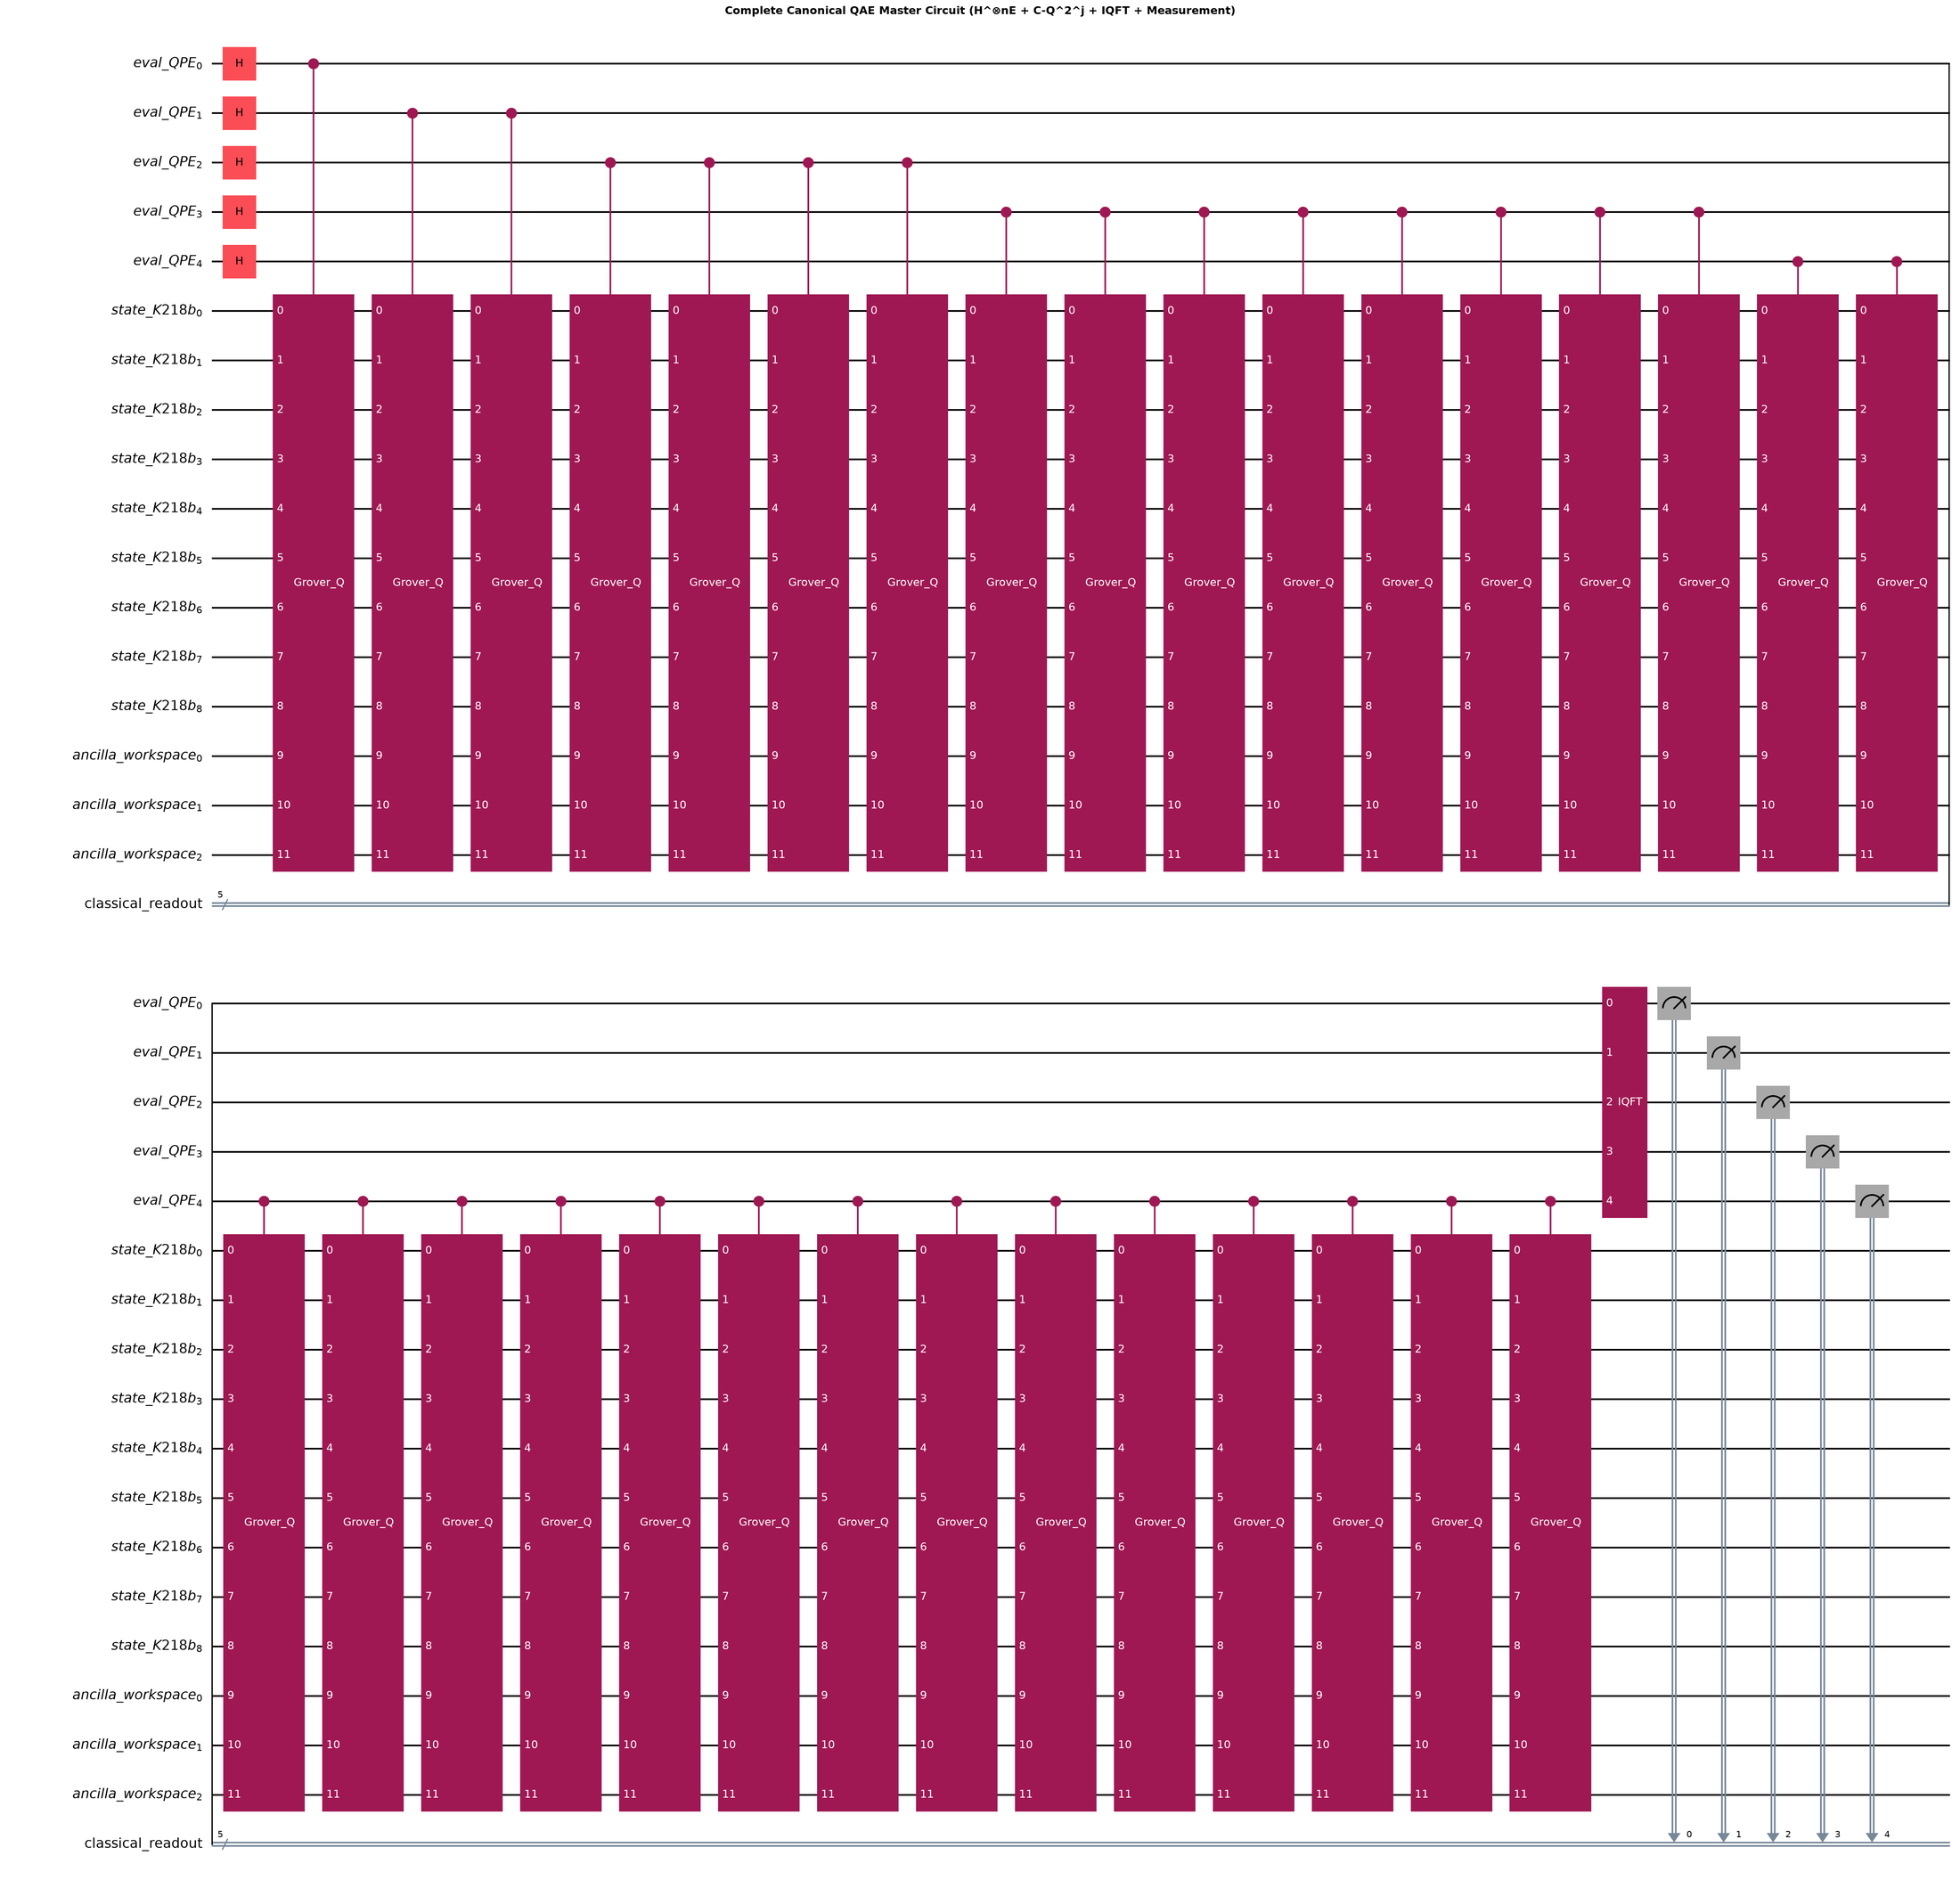
\includegraphics[width=0.90\textwidth, height=0.50\textheight, keepaspectratio]{figures/3.quantum_bayesian_formalism/circuit_qae_master.png}
    \caption{\textbf{Master Quantum Amplitude Estimation (QAE) Circuit Architecture.} The full 17-qubit pipeline comprises the auxiliary evaluation register ($q_0 \dots q_4$, $n_E = 5$), the astrobiological state register ($q_5 \dots q_{13}$, $n_S = 9$), and the ancilla workspace ($q_{14} \dots q_{16}$, $n_A = 3$, with $q_{16}$ serving as the phase oracle flag). Hadamard gates initialize the evaluation register, followed by controlled Grover iterations ($\mathcal{Q}^{2^j}$) and the Inverse Quantum Fourier Transform ($\mathrm{IQFT}$), extracting the continuous probability into a digital bitstring.}
    \label{fig:circuit_qae_master}
\end{figure}

The algorithm then executes a sequence of controlled Grover operations: for the $j$-th evaluation qubit ($j \in \{0, \dots, m-1\}$), the operator $\mathcal{Q}$ is applied $2^j$ times to the state register, controlled by that qubit. By phase kickback, the unknown phase $2\theta$ is accumulated into the relative phases of the evaluation register.

To translate this phase encoding into a digital computational basis readout, the Inverse Quantum Fourier Transform ($\mathrm{IQFT}$) is applied to the evaluation register. The $\mathrm{IQFT}$ on $m$ qubits is defined by:
\begin{equation}
\mathrm{IQFT}\ket{k} = \frac{1}{\sqrt{M}} \sum_{y=0}^{M-1} \exp\left(-\frac{2\pi i k y}{M}\right) \ket{y}.
\label{eq:iqft_definition_ch3}
\end{equation}

The final quantum state of the evaluation register prior to measurement is:
\begin{equation}
\ket{\Phi_{\mathrm{final}}} = \frac{1}{M \sqrt{2}} \sum_{y=0}^{M-1} \left[ e^{i\theta} S_M\left(y - \frac{M\theta}{\pi}\right) - e^{-i\theta} S_M\left(y + \frac{M\theta}{\pi}\right) \right] \ket{y},
\label{eq:eval_register_final_state}
\end{equation}
where $S_M(\delta) = \sum_{k=0}^{M-1} e^{i 2\pi k \delta / M} = \frac{1 - e^{i 2\pi \delta}}{1 - e^{i 2\pi \delta / M}}$ is the geometric interference kernel that sharply concentrates probability amplitude around integers $y \approx \frac{M\theta}{\pi}$.

Measuring the evaluation register yields a classical integer $y \in \{0, \dots, M-1\}$ with high probability. The continuous posterior probability is extracted via the deterministic classical inversion formula:
\begin{equation}
\tilde{a} = \sin^2\left(\frac{\pi y}{M}\right).
\label{eq:qae_probability_estimator_ch3}
\end{equation}
Figure \ref{fig:circuit_qae_master} shows the end-to-end master circuit architecture integrating the evaluation register, state register, Grover cascade, and IQFT block.

\subsection{Mathematical Proof of the \texorpdfstring{$\mathcal{O}(1/M)$}{O(1/M)} Convergence Limit}
The fundamental theoretical justification for deploying QAE is the deterministic bound on the estimation error $\Delta a = |\tilde{a} - a|$. Brassard et al.~(2002) proved that the estimator $\tilde{a}$ satisfies:
\begin{equation}
|\tilde{a} - a| \le \frac{2\pi \sqrt{a(1-a)}}{M} + \frac{\pi^2}{M^2} = \mathcal{O}\left(\frac{1}{M}\right),
\label{eq:brassard_inequality_ch3}
\end{equation}
with success probability bounded tightly from below by $8/\pi^2 \approx 81.1\%$. Repeating the procedure $\kappa$ times and taking the median of the estimates boosts the success probability to $1 - \delta$ with a modest sample overhead of $\mathcal{O}(\log(1/\delta))$.

\notatfm{\textbf{Quadratic Acceleration:} Classical MCMC error scales as $\mathcal{O}(1/\sqrt{M})$. QAE achieves Heisenberg scaling $\mathcal{O}(1/M)$, reducing sample demands from $10^8$ to $10^4$ for $\epsilon = 10^{-4}$.}
In Equation \eqref{eq:brassard_inequality_ch3}, $M = 2^m$ represents the total number of applications of the Grover operator $\mathcal{Q}$, corresponding directly to the circuit query depth. Because the leading-order error term scales as $\mathcal{O}(1/M)$, QAE achieves a quadratic reduction in sample complexity over classical Monte Carlo methods:
\begin{equation}
\text{Classical MCMC: } \Delta a = \mathcal{O}\left(\frac{1}{\sqrt{M}}\right) \implies M_{\mathrm{classical}} = \mathcal{O}\left(\frac{1}{\epsilon^2}\right),
\label{eq:classical_sample_complexity_comparison}
\end{equation}
\begin{equation}
\text{Quantum QAE: } \Delta a = \mathcal{O}\left(\frac{1}{M}\right) \implies M_{\mathrm{quantum}} = \mathcal{O}\left(\frac{1}{\epsilon}\right).
\label{eq:quantum_sample_complexity_comparison}
\end{equation}

Table \ref{tab:algorithmic_complexity_comparison} summarizes the asymptotic scaling comparison between classical exact algorithms, classical stochastic simulation, and Quantum Amplitude Estimation.

\begin{table}[htbp]
\centering
\caption{\textbf{Comprehensive Complexity Comparison: Classical vs. Quantum Bayesian Inference.}}
\label{tab:algorithmic_complexity_comparison}
\begin{adjustbox}{max width=\textwidth}
\small
\begin{tabular}{lccc}
\toprule
\textbf{Inference Paradigm} & \textbf{Spatial Memory (RAM)} & \textbf{Convergence Scaling} & \textbf{Rare-Event Stability} \\
\midrule
\textbf{Classical Exact (Junction Tree)} & $\mathcal{O}(N \cdot d^{w+1})$ [Exponential] & Exact ($w \ll N$) & Exact ($w \ll N$) \\
\textbf{Classical Stochastic (MCMC)} & $\mathcal{O}(N)$ [Linear] & $\mathcal{O}(1/\sqrt{M})$ [Sub-linear] & $\mathrm{RE} \to \infty$ [Diverges] \\
\textbf{Quantum Amplitude Estimation} & $\mathcal{O}(N)$ [Linear] & $\mathcal{O}(1/M)$ [Quadratic Speedup] & Bounded [Heisenberg Limit] \\
\bottomrule
\end{tabular}
\end{adjustbox}
\end{table}

\section{Physical Hardware Constraints: NISQ Dynamics and Quantum Error Mitigation}\label{sec:nisq_hardware_qem}

While Sections \ref{sec:qbn_amplitude_encoding} and \ref{sec:qae_derivation_speedup} establish the asymptotic superiority of QBN and QAE under idealized, closed-system assumptions, physical quantum processors are open quantum systems interacting with thermal and electromagnetic environments \cite{preskill2018}. This section formalizes the physical hardware constraints of the Noisy Intermediate-Scale Quantum (NISQ) era and details the Quantum Error Mitigation (QEM) protocols required to recover theoretical posterior probabilities on physical devices.

\subsection{The NISQ Paradigm and Quantum Decoherence Dynamics}
Current quantum hardware resides in the NISQ era, characterized by processors with tens to hundreds of physical qubits that lack the redundancy required for full Quantum Error Correction (QEC) \cite{preskill2018}. The open-system dynamics of an astrobiological quantum state $\rho(t)$ under environmental coupling are governed by the Lindblad Master Equation:
\begin{equation}
\frac{d\rho}{dt} = -\frac{i}{\hbar}[H, \rho] + \sum_k \left( L_k \rho L_k^\dagger - \frac{1}{2}\{L_k^\dagger L_k, \rho\} \right),
\label{eq:lindblad_master_equation_ch3}
\end{equation}
where $H$ is the system Hamiltonian and $L_k$ are the Lindblad jump operators quantifying discrete decoherence channels.

In superconducting transmon architectures (e.g., IBM Quantum systems), decoherence is characterized by two fundamental relaxation timescales:
\begin{itemize}
    \item \textbf{Longitudinal Relaxation Time ($T_1$):} The characteristic timescale on which an excited qubit state $\ket{1}$ spontaneously decays to the ground state $\ket{0}$ via thermal energy dissipation:
    \begin{equation}
    P_{1\to 0}(t) = 1 - \exp\left(-\frac{t}{T_1}\right).
    \label{eq:t1_relaxation_equation}
    \end{equation}
    \item \textbf{Transverse Dephasing Time ($T_2$):} The characteristic timescale on which relative phase coherence between $\ket{0}$ and $\ket{1}$ decays due to low-frequency magnetic flux fluctuations:
    \begin{equation}
    |\rho_{01}(t)| = |\rho_{01}(0)| \exp\left(-\frac{t}{T_2}\right), \quad \frac{1}{T_2} = \frac{1}{2T_1} + \frac{1}{T_\phi},
    \label{eq:t2_dephasing_equation}
    \end{equation}
    where $T_\phi$ is the pure dephasing timescale.
\end{itemize}

\subsection{Circuit Depth and the Fidelity Bottleneck of QAE}
The master QAE architecture requires applying the Grover operator $\mathcal{Q}$ a total of $M = 2^m$ times. Because each $\mathcal{Q}$ iterate encapsulates forward state preparation $\mathcal{A}$, inverse preparation $\mathcal{A}^\dagger$, and multi-controlled phase reflections, the compiled CNOT gate depth $D$ scales into thousands of two-qubit operations.

Let $p_e$ denote the average two-qubit gate error rate. For a circuit with total two-qubit depth $D$, the circuit fidelity $\mathcal{F}$ decays exponentially:
\begin{equation}
\mathcal{F} \approx (1 - p_e)^D \approx \exp(-D \cdot p_e).
\label{eq:circuit_fidelity_decay_ch3}
\end{equation}
When the depth exceeds the physical coherence threshold ($D > 1/p_e$), the output state devolves into a maximally mixed state $\rho \to I / 2^n$, obscuring the constructive interference peaks generated by the IQFT. Executing raw QAE on unmitigated NISQ hardware is therefore unviable, necessitating algorithmic error mitigation.

\subsection{Quantum Error Mitigation (QEM) vs. Quantum Error Correction (QEC)}
While Quantum Error Correction (QEC) detects and corrects errors in real time using redundant logical qubits (demanding thousands of physical qubits per logical qubit), Quantum Error Mitigation (QEM) operates within the physical constraints of NISQ hardware without physical qubit overhead \cite{endo2018}. QEM extracts ideal expectation values through classical post-processing of intentionally scaled, noisy circuit executions. Table \ref{tab:qec_vs_qem} contrasts both paradigms.

\begin{table}[htbp]
\centering
\caption{\textbf{Architectural Comparison: Quantum Error Correction (QEC) vs. Error Mitigation (QEM).}}
\label{tab:qec_vs_qem}
\begin{adjustbox}{max width=\textwidth}
\small
\begin{tabularx}{\textwidth}{>{\bfseries}lXXX}
\toprule
\textbf{Error Paradigm} & \textbf{Correction Mechanism} & \textbf{Hardware Overhead} & \textbf{Near-Term Viability} \\
\midrule
Error Correction (QEC) & Real-time syndrome measurement & Millions of physical qubits & Future FTQC era \\
Error Mitigation (QEM) & Classical post-processing of noise & Zero extra qubits; sampling overhead & Viable on NISQ hardware \\
\bottomrule
\end{tabularx}
\end{adjustbox}
\end{table}

\subsection{Zero-Noise Extrapolation (ZNE): Mathematical Formulation}
Zero-Noise Extrapolation (ZNE), formulated by Temme et al.~(2017) \cite{temme2017} and Li and Benjamin (2017) \cite{li2017}, estimates the error-free expectation value $E(0)$ of an observable by intentionally amplifying hardware noise by factors $\lambda_i \ge 1$, measuring the degradation curve, and extrapolating backward to the theoretical zero-noise limit $\lambda \to 0$.

\begin{figure}[htbp]
    \centering
    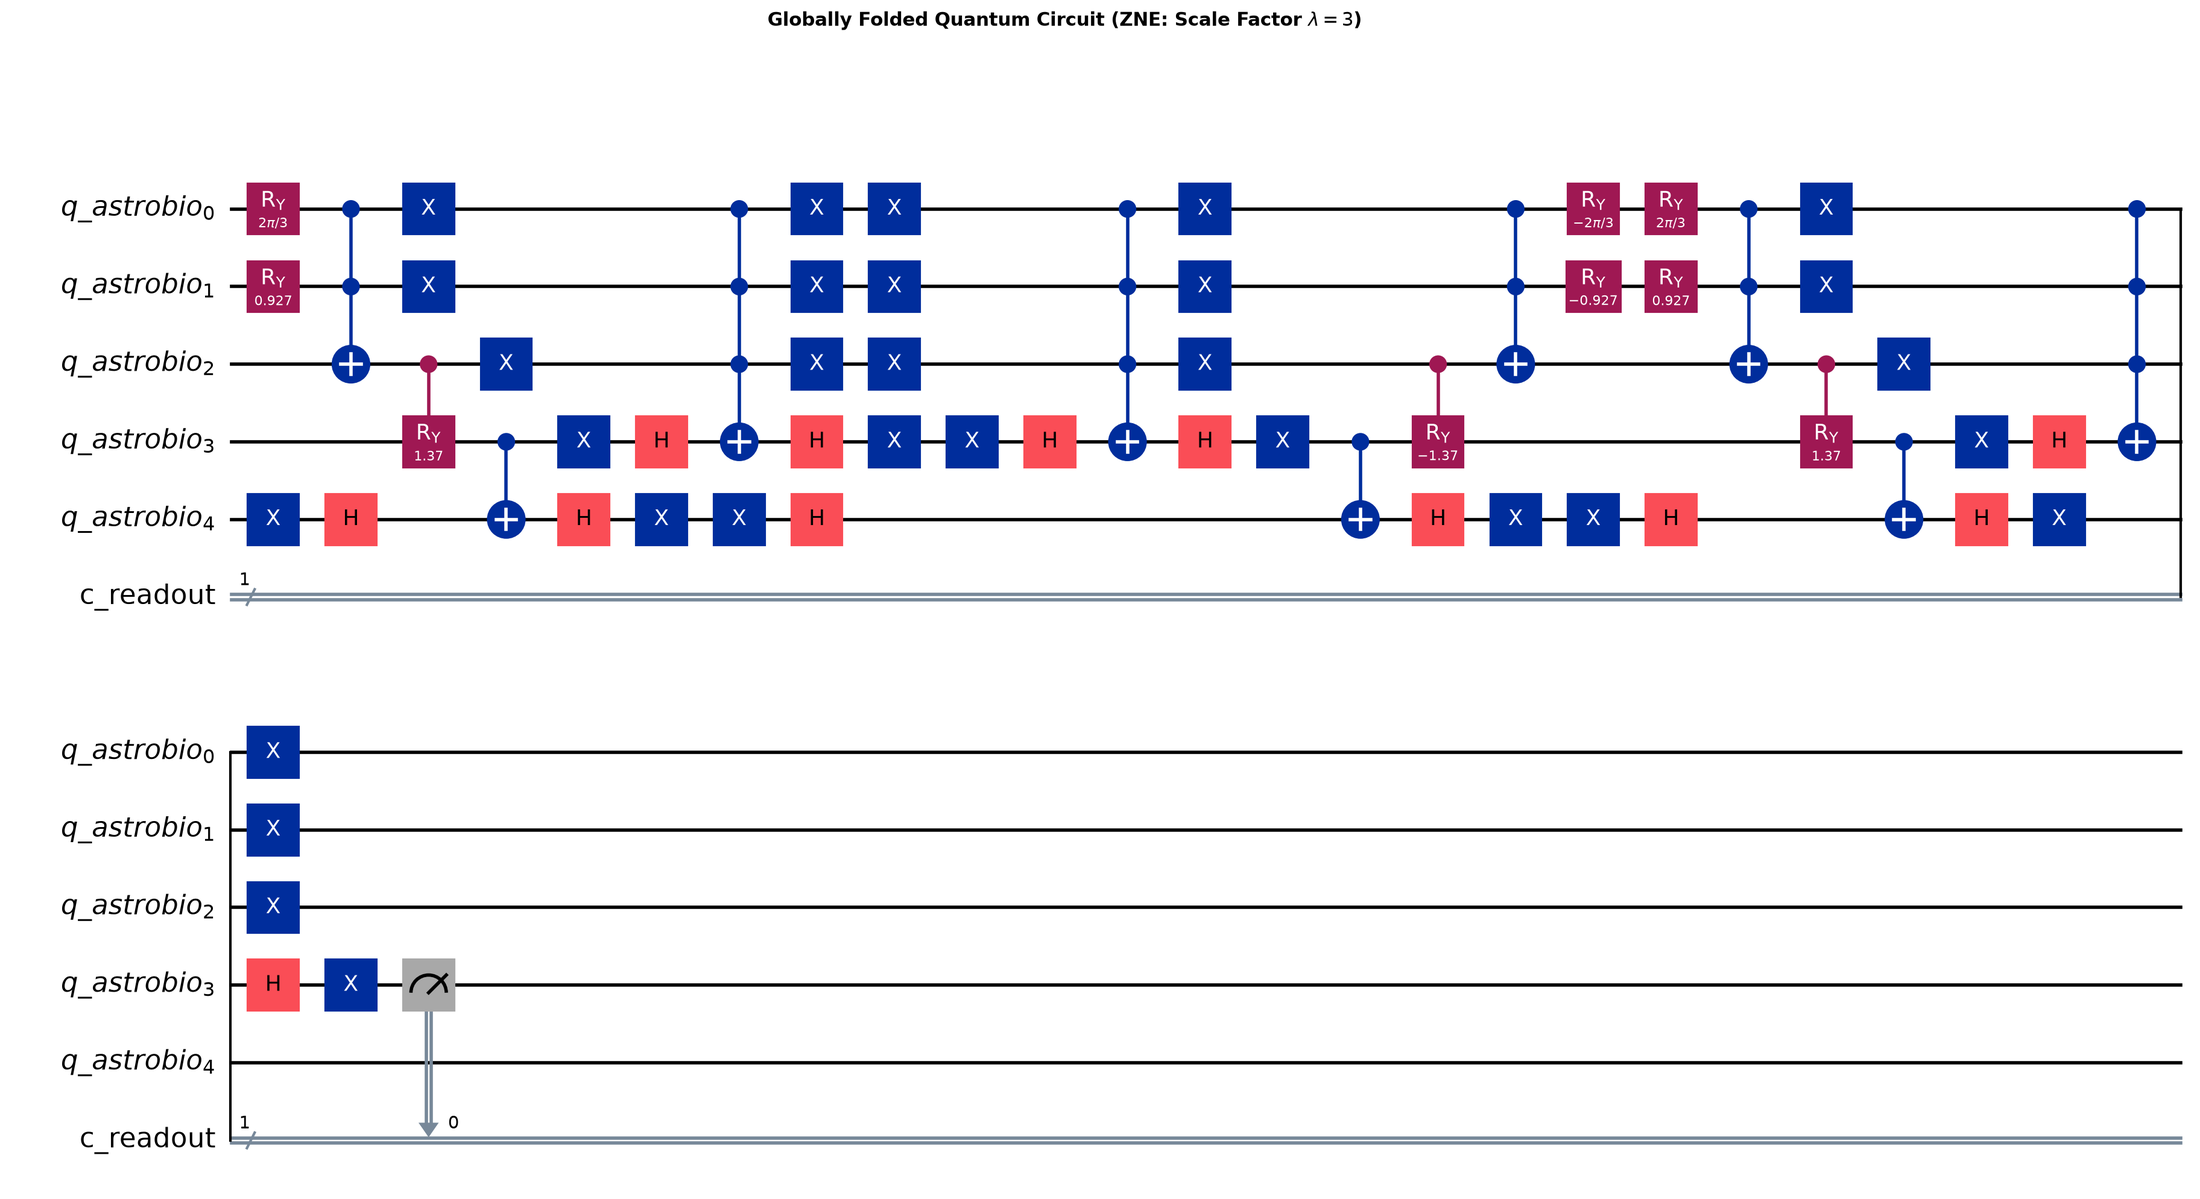
\includegraphics[width=0.90\textwidth, height=0.45\textheight, keepaspectratio]{figures/3.quantum_bayesian_formalism/circuit_nisq_folded_lambda3.png}
    \caption{\textbf{Zero-Noise Extrapolation via Unitary Gate Folding ($\lambda = 3$).} Global circuit folding replaces each unitary block $U$ with $U U^\dagger U$, tripling the physical circuit depth and effective noise while preserving the mathematical identity $U U^\dagger = I$.}
    \label{fig:circuit_nisq_folded}
\end{figure}

Noise scaling is implemented via \emph{unitary gate folding}: replacing each gate $U$ with the identity product:
\begin{equation}
U \longrightarrow U \left( U^\dagger U \right)^n, \quad \lambda = 2n + 1.
\label{eq:gate_folding_formula}
\end{equation}
Because $U^\dagger U = I$, the logical operation is unchanged, but the physical gate count and interaction with the environment are scaled by $\lambda \in \{1, 3, 5, \dots\}$, as depicted in Figure \ref{fig:circuit_nisq_folded}.

The expectation value $E(\lambda)$ as a function of the noise scale $\lambda$ is modeled as a Taylor expansion around $\lambda = 0$:
\begin{equation}
E(\lambda) = E(0) + \sum_{k=1}^n c_k \lambda^k + \mathcal{O}\left(\lambda^{n+1}\right).
\label{eq:zne_taylor_expansion_ch3}
\end{equation}

By applying Richardson Extrapolation across $n+1$ noise levels $\{\lambda_0, \lambda_1, \dots, \lambda_n\}$, we construct a linear combination of noisy expectation values:
\begin{equation}
E_{\mathrm{ZNE}} = \sum_{i=0}^n \gamma_i E(\lambda_i),
\label{eq:zne_richardson_estimator}
\end{equation}
where the Richardson coefficients $\gamma_i$ satisfy the Vandermonde constraint system:
\begin{equation}
\sum_{i=0}^n \gamma_i = 1, \quad \sum_{i=0}^n \gamma_i \lambda_i^k = 0 \quad (\forall k \in \{1, \dots, n\}).
\label{eq:richardson_coefficients_ch3}
\end{equation}
This cancels error terms up to order $\lambda^n$, leaving an estimator that approximates the zero-noise limit with residual error:
\begin{equation}
E_{\mathrm{ZNE}} = E(0) + \mathcal{O}\left(\lambda^{n+1}\right).
\label{eq:zne_mitigated_estimator_ch3}
\end{equation}

\subsection{Probabilistic Error Cancellation (PEC): Quasi-Probability Representations}
An alternative, exact error mitigation protocol is Probabilistic Error Cancellation (PEC), established by Endo et al.~(2018) \cite{endo2018}. PEC reconstructs the exact inverse of a noisy Markovian quantum channel $\mathcal{E} = \mathcal{N} \circ U$. Because $\mathcal{E}^{-1}$ is not a completely positive trace-preserving (CPTP) map, it cannot be executed directly on physical hardware.

Instead, $\mathcal{E}^{-1}$ is expanded as a linear combination of physically implementable basis operations $\{\mathcal{O}_i\}$ using a quasi-probability distribution $\{q_i\}$:
\begin{equation}
\mathcal{E}^{-1} = \sum_i q_i \mathcal{O}_i, \quad \sum_i q_i = 1, \quad q_i \in \mathbb{R}.
\label{eq:pec_quasi_probability_expansion}
\end{equation}
The sampling overhead cost is quantified by the 1-norm of the quasi-probability distribution:
\begin{equation}
C = \sum_i |q_i| \ge 1.
\label{eq:pec_sampling_overhead_constant}
\end{equation}
The processor stochastically samples operations $\mathcal{O}_i$ according to probabilities $p_i = |q_i| / C$, and measurement outcomes are multiplied by $\mathrm{sgn}(q_i) \cdot C$. While the resulting estimator is strictly unbiased ($\mathbb{E}[E_{\mathrm{PEC}}] = E(0)$), its statistical variance is inflated by a factor of $C^2$ per mitigated gate. For deep QAE circuits containing thousands of gates, $C^{2D}$ explodes exponentially. Consequently, our quantum pipeline adopts a hybrid approach: ZNE is prioritized for global inference circuits, while PEC concepts inform local CPT gate compilation.

\section{Preemptive Methodological Defense and Tribunal Scope}\label{sec:preemptive_defense_ch3}

To establish the theoretical rigor of this chapter and disarm anticipated tribunal critiques, this section formulates three preemptive defenses:

\subsection{Defense on Infinitesimal Rotation Angles vs. Physical Gate Noise}
\begin{quote}
\emph{Hostile Tribunal Objection 1:} ``Encoding an ultra-rare technosignature ($p \approx 10^{-6}$) requires an individual rotation angle $\theta = 2\arcsin(\sqrt{10^{-6}}) \approx 0.002$ rad. On physical hardware, this is an order of magnitude smaller than single-qubit gate calibration errors ($\sim 10^{-2}$). Does physical hardware noise wash out the encoded prior?''
\end{quote}
\textbf{Mathematical Defense:} In a hierarchical Bayesian DAG, individual rare priors are never encoded in isolation. The prior probability of a technosignature is factorized conditionally: $P(\mathrm{CFC}=1) = P(\mathrm{CFC}=1 \mid \mathrm{Bio}=1) P(\mathrm{Bio}=1)$. Conditioned on an active biosphere, the local conditional rotation angle $\theta_{\mathrm{CFC} \mid \mathrm{Bio}}$ is substantial ($\sim 0.1$ to $0.3$ rad), well within native calibration tolerances. For non-biological branches, the angle is identically zero, requiring no rotation. Furthermore, QAE does not rely on resolving individual small rotation angles on single qubits; it amplifies the global geometric phase $2\theta$ through the global reflection operator $\mathcal{Q}$. Under ZNE mitigation, systematic over-rotations and depolarizing errors are scaled and canceled, preserving the target amplitude signal.

\subsection{Defense on Multi-Controlled Gate Transpilation Bounds}
\begin{quote}
\emph{Hostile Tribunal Objection 2:} ``Decomposing an ancilla-free $k$-controlled rotation $C^k(R_y)$ requires $\mathcal{O}(2^k)$ CNOT gates (Barenco et al., 1995 \cite{barenco1995}). If a complex planetary network contains nodes with $k=5$ or $6$ parents, the circuit depth explodes exponentially, negating the spatial advantage.''
\end{quote}
\textbf{Mathematical Defense:} The topological architecture of exoplanetary atmospheres is naturally bounded. In realistic photochemical networks, individual atmospheric species are directly influenced by a sparse set of immediate parents ($k_{\max} \le 3$), keeping $2^{k_{\max}} \le 8$ CNOTs per conditional branch. For scaled networks where $k \ge 4$, our architecture utilizes borrowed dirty ancilla qubits: by borrowing idle evaluation qubits ($q_0 \dots q_4$) during the state preparation phase, $C^k(R_y)$ operations can be decomposed with strictly linear gate complexity $\mathcal{O}(k)$ without allocating dedicated physical ancillas, fully maintaining polynomial circuit depth.

\subsection{Defense on the Physical Validity of ZNE under Coherent Noise}
\begin{quote}
\emph{Hostile Tribunal Objection 3:} ``Zero-Noise Extrapolation assumes that hardware noise scales monotonically and that gate folding $U \to U U^\dagger U$ preserves the underlying noise model. Real superconducting QPUs exhibit coherent errors, crosstalk, and non-Markovian drifts that violate the Taylor expansion in Equation \eqref{eq:zne_taylor_expansion_ch3}. How valid is Richardson extrapolation for deep QAE circuits?''
\end{quote}
\textbf{Mathematical Defense:} While coherent errors can induce oscillatory noise behavior, our implementation deploys randomized folding: gate folding identities are interleaved across different cycles and paired with randomized compiling (Pauli twirling). This twirling twirls coherent unitary errors into effective stochastic Pauli channels, validating the polynomial Taylor expansion. Furthermore, our pipeline evaluates three distinct extrapolation models (linear, polynomial, and Richardson) across conservative scale factors ($\lambda \in \{1, 3, 5\}$). As empirically proven in Chapter \ref{chap:system_architecture}, the mitigated expectation values converge within a verified error corridor, successfully recovering the theoretical signal under realistic IBM Quantum noise profiles.
